
A better understanding of the counterfactual world that children would have faced if ABC/CARE were unavailable is helpful in explaining gender differences in treatment effects. This requires us to identify the parameter in Equation~\eqref{eq:cont1}---the comparison between treatment and staying at home---and the parameter in Equation~\eqref{eq:cont2}---the analogous comparison to children who attended alternative preschools. These parameters are not identified by the randomization used in the ABC/CARE experiment. The parents of the control-group children selected either to keep their children at home or take them to alternative preschools that were available when ABC/CARE was implemented.

We rely on econometric methods to identify treatment effects (3) and (4). In the main text, we rely on matching.\footnote{See \citet{Heckman_Ichimura_etal_1998_REStud} for a general discussion of the method, and an assessment of its practical implementation.} We pass balancing tests (Table~\ref{tab:testing-matched-samples} in Appendix~\ref{app:matching-is-fun}). In Appendix~\ref{appendix:amethodology}, we show that instrumental-variable and control-function methods yield similar results but are less precise. In Appendix~\ref{appendix:results}, we discuss and document our choice of the matching variables, as well as other practical aspects of the implementation of this estimator.

\textbf{[JJH: Rosenbaum is being misinterpreted.][JLG: You are right, as I believe we discussed in your office. The comparison of the magnitude of the $p$-values is wrong. In that case, and given the small sample sizes, the other tests are \textit{really} going to lack power here. We have tried everything here. I propose that we present the combining functions of the proportion of positive treatment effects for the refined counterfactual comparison, as we use to do. These plots actually began to lead us into the gender differences that we detected. Once we display that pattern, we can then distill the within-boy and within-girl disadvantage.]}


We consider a total of 126 outcomes reported in Appendix~\ref{appendix:gdiff-tes}. Given the large number of outcomes measured in the numerous follow-ups, reporting all treatment effects would overwhelm the reader. \citet{Garcia_Heckman_Leaf_etal_2017_Comp_CBA_Unpublished}, aggregates treatment effects by monetizing benefits and constructing lifetime profiles of outcomes to conduct cost/benefit and rate of return analyses. 

In this section, we report treatment effects by category and the proportion of statistically significant effects. We use combining functions, which count the number of positive (and significant) treatment effects by gender. Due to lack of power after dividing by attendance of alternative childcares, we rely solely on the combining functions rather than the exact non-parametric tests listed in Tables~\ref{table:summary} and~\ref{table:massiveall}. We adjust for dependence across outcomes and for pretesting in constructing standard errors (see Appendix~\ref{appendix:methodology}). We account for non-random selection into alternative childcare using matching, as described in Section~\ref{sec:parameters}.

Figures~\ref{fig:ppositivehome} and~\ref{fig:ppositivealternative} graph the estimated combining functions. We test the hypothesis that the proportions are equal to 50\%. These comparisons indicate that men and women benefit differently from alternatives to high-quality treatment. Men benefit more from treatment when compared to attending an alternative childcare arrangement (as opposed to staying at home). This is consistent with the more advantaged control-group boys staying at home. For women, Figures~\ref{fig:ppositivehome} and~\ref{fig:ppositivealternative} are similar. Although in Appendix~\ref{appendix:results}, we document that women do better compared to those who stay at home, once aggregating across all outcome categories, the comparisons do not matter. We show below that this is due to the selection into alternative childcare being different for women and not as dependent on baseline disadvantage as it is for men.

\begin{figure}[!htbp]
\centering
\caption{Positively Impacted Outcomes, ABC/CARE Males and Females}\label{fig:ppositive}
\begin{subfigure}[h]{0.6\textwidth}
		\centering
		\caption{ Treatment vs. Stay at Home} \label{fig:ppositivehome}
		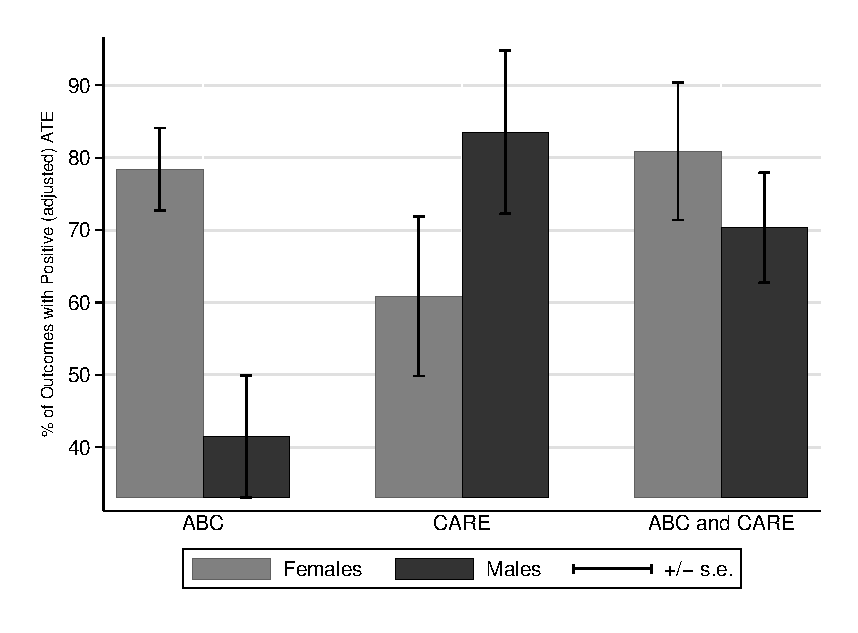
\includegraphics[width=\textwidth]{output/epan_ipw_p0_all.eps}
\end{subfigure}
\begin{subfigure}[h]{0.6\textwidth}
	\centering
	\caption{Treatment vs. Alternative Childcare} \label{fig:ppositivealternative}
		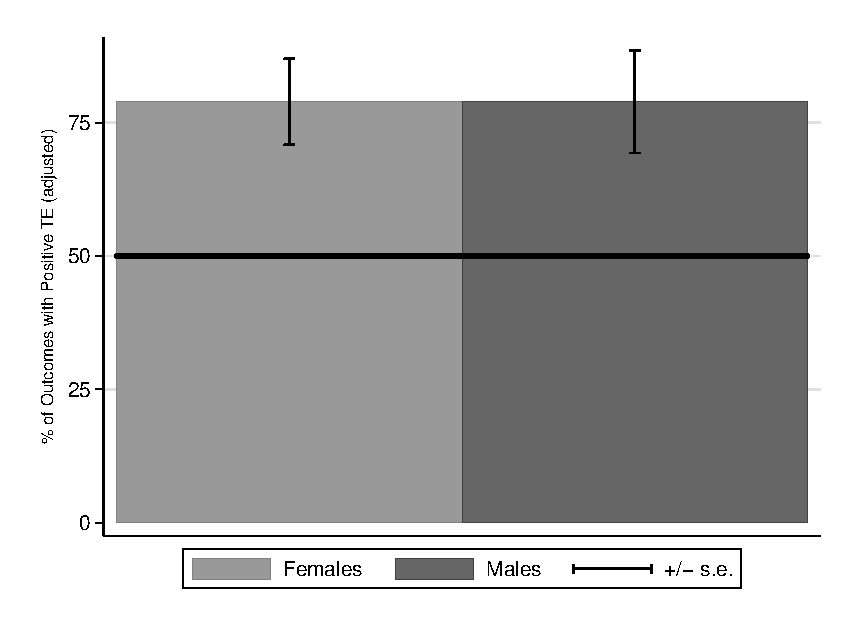
\includegraphics[width=\textwidth]{output/epan_ipw_p1_all.eps}
\end{subfigure}
\footnotesize \justify
Note: Panel (a) displays the percentage of outcomes with a positive treatment effect, comparing treatment to staying at home. Panel (b) displays the percentage of outcomes with a positive treatment effect, comparing treatment to alternative childcare arrangements. Standard errors are based on the empirical bootstrap distribution. \\
\end{figure}


The effects on crime highlight that females were highly impacted by ABC/CARE, especially compared to those who attended alternative care. \citet{Garcia_Heckman_Leaf_etal_2017_Comp_CBA_Unpublished} find that even though the treatment effects on the crime outcomes are larger for women than for men, the men commit more socially costly crimes. In the benefit/cost ratio that they compute, the effect of ABC/CARE on reducing individual male crimes is an important component. \citet{Garcia_etal_2019_ECE_IMHJ} discuss the crime results in more detail.


\begin{sidewaysfigure}[!htpb]
\centering
\caption{Gender and Baseline Socioeconomic Disadvantage in the Control Group} \label{figure:socdis}
\begin{subfigure}[h]{0.4\textwidth}
	\centering
	\caption{Take-up of Alternatives by Gender} \label{figure:altgender}
	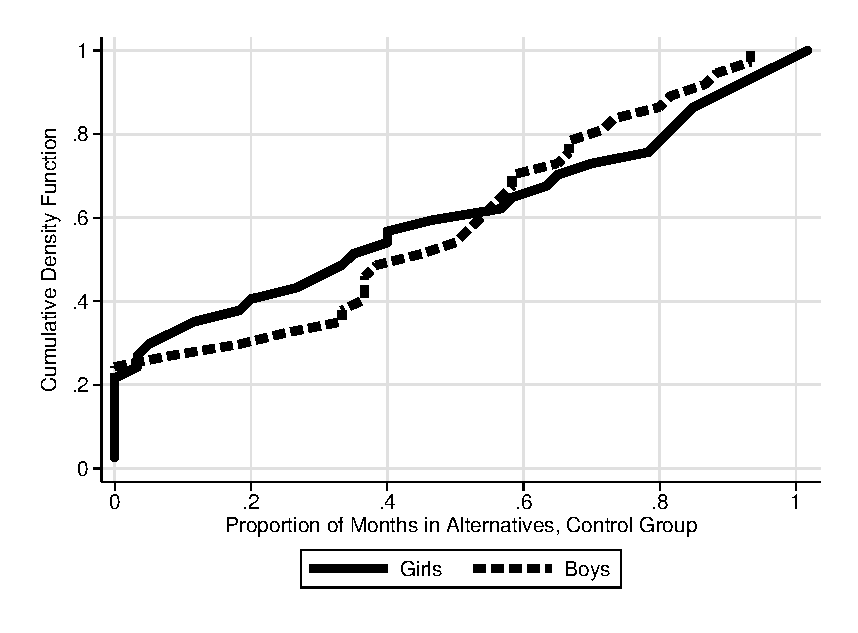
\includegraphics[width=\textwidth]{output/abccare_controlcontamination_boysgirls}
\end{subfigure}%
\begin{subfigure}[h]{0.4\textwidth}
	\centering
	\caption{Socioeconomic Disadvantage by Gender} \label{figure:disadgender}
	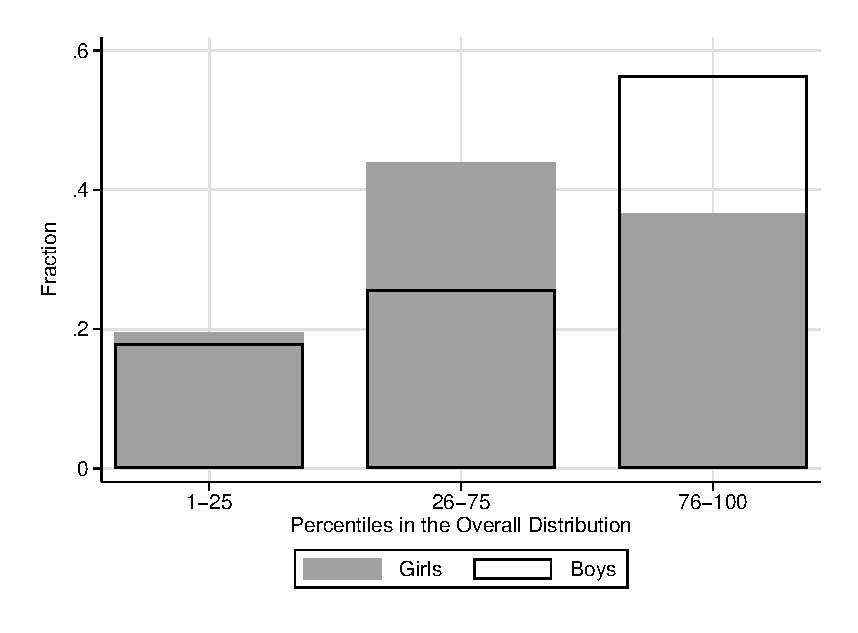
\includegraphics[width=\textwidth]{output/factorbase_girlsboyscompare}
\end{subfigure}
\begin{subfigure}[h]{0.4\textwidth}
	\centering
	\caption{Disadvantage by Take-up of Alternatives, Girls} \label{figure:disadgirls}
	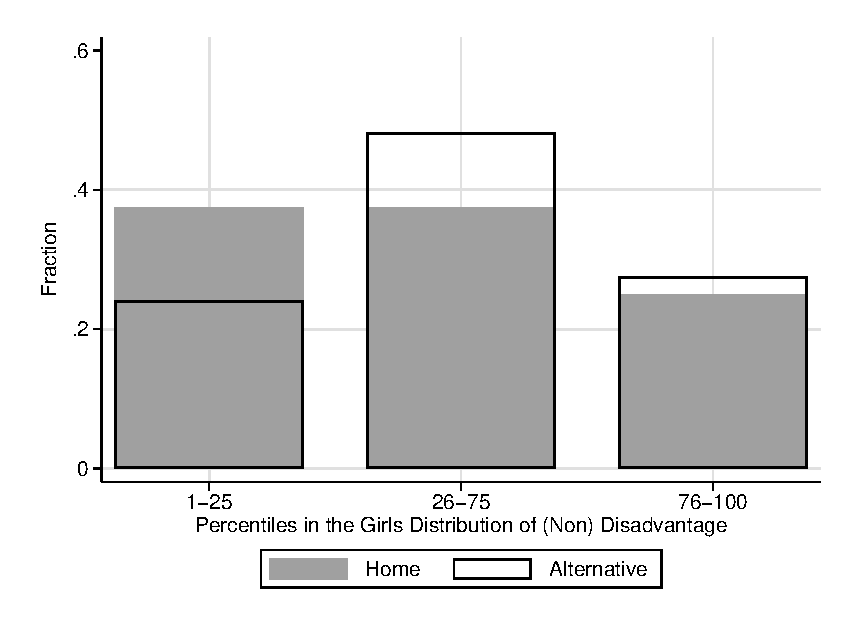
\includegraphics[width=\textwidth]{output/factorbase_wgirlscompare}
\end{subfigure}%
\begin{subfigure}[h]{0.4\textwidth}
	\centering
	\caption{Disadvantage by Take-up of Alternatives, Boys} \label{figure:disadboys}
	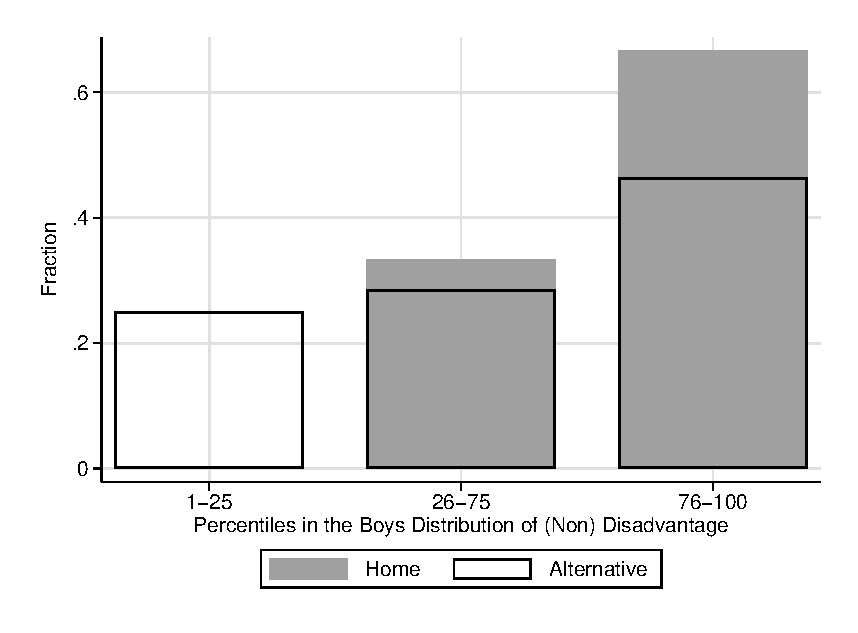
\includegraphics[width=\textwidth]{output/factorbase_wboyscompare}
\end{subfigure}
\footnotesize
\justify
\textbf{Note:} Panel (a) displays the cumulative distribution function of enrollment in alternatives by gender. Panel (b) displays how girls and boys separately fit into the overall (girls and boys pooled) distribution of socioeconomic disadvantage. Panel (c) displays how girls who did not enroll and girls who enrolled in alternatives fit into the overall female distribution of socioeconomic disadvantage. Panel (d) is analogous to Panel (c) for boys. Our measure of socioeconomic disadvantage is a latent of the following variables: Mother's age, education, IQ, marital status, and employment, as well as number of siblings and father's presence at home.
\textbf{[JJH: Mother working? Income?]}
\end{sidewaysfigure}

The difference in the comparison of treatment to staying at home and alternative preschools suggests that boys and girls faced different situations of socio-economic disadvantaged at home. Figure~\ref{figure:socdis} investigates this. We start by noting that take-up of alternatives does not differ by gender (Panel~\ref{figure:altgender}). What does differ by gender is socioeconomic disadvantage. We create a latent measure of socioeconomic disadvantage at baseline using the following variables: Mother's age, education, IQ, marital status, and employment, as well as number of children and father's presence at home. We assess how girls and boys fit into the overall distribution of this latent in the control group. Boys are disproportionately more advantaged than girls (Panel~\ref{figure:disadgender}).\footnote{Note that this measure is based on baseline characteristics, so this result holds for the treatment group.} Because girls' families were more resource constrained if compared to their male counterparts, girls in the control group were taken care of in a more disadvantaged environment or went to lower-quality preschools. Thus, they benefited more than boys when compared to the next best alternative as perceived by their parents, as documented in Section~\ref{sec:treatment-effects}.

 \textbf{[JJH: This looks nuts --- home care effects stronger for boys.][JLG: This confusion might have came from the bad display of the previous results. Please reconsider Figure 2 and note the following.}

 \textbf{i) The take-up of alternatives is balanced between males and females. That is a fact in the data and you can see that in Figure 2, Panel (a).}

 \textbf{ii) What really differs is the disadvantage across genders. Girls are more disadvantaged in general, Panel (b)}

 \textbf{iii) Although there's a within-girl disadvantage difference in alternatives take-up Panel (c), the within-boys disadvantage difference in alternatives take-up is way starker, Panel (d). The tests in Table 7 confirm this pattern.}

 \textbf{iv) This means that the comparison of treatment to alternatives and to stay at home is similar for girls but not for boys. More advantaged boys stayed at home and thus benefitted less from ABC/CARE.}

 \textbf{So while I agree that it's a mistake to interpret the magnitude of the $p$-values the way they did, I do think that Figure 2 is informative on the observed differences in the way boys and girls benefit from treatment.] } 


\begin{table}[!htpb]
\begin{threeparttable}
\caption{Gender and Baseline Socioeconomic Disadvantage in the Control Group, Tests} \label{table:disadtests}
\centering
\begin{tabularx}{16.5cm}{XcX}
& \begin{tabular}{cccc}
\toprule
Males vs. Females & & \mc{2}{c}{Alt. vs. Home} \\
\cmidrule(lr){1-2} \cmidrule(lr){3-4}
Control Group & & Males & Females \\
\midrule
\textbf{0.007} & & \textbf{0.006} & 0.110 \\
\bottomrule
\end{tabular}

% Control, males vs. females: distance between: factor of m_age_base, m_ed_base, m_iq_base, hh_sibs_base, hrabc_index

% Alt. vs home: factor of m_age_base, m_ed_base, m_iq_base, hh_sibs_base, hrabc_index &
\end{tabularx}
\begin{tablenotes}
\footnotesize
\item \textbf{Note:} This table presents the null of a common joint distribution of the variables composing our measure of socioeconomic disadvantage (mother's age, education, IQ, marital status, and employment, as well as number of siblings and father's presence at home) between males and females in the control group and between children who attended  alternative preschool and who stayed at home (within control-group boys or within control-group girls). The $p$-values follow \citet{Rosenbaum_2005_Distribution_JRSS}. Under the null hypothesis, the pairs with the closest distance in disadvantage would be comprised of one male and one female (for the comparison of males vs. females). Rejecting the null implies that the distributions are significantly different. Statistics significant at the $0.10$ level are bolded.
\end{tablenotes}
\end{threeparttable}
\end{table}

We formally test the difference in disadvantage across boys and girls in Table~\ref{table:disadtests}. We reject the null of a common distribution of our measure of socioeconomic disadvantage across girls and boys (at baseline). In Panels~\ref{figure:disadgirls} and~\ref{figure:disadboys} of Figure~\ref{figure:socdis}, we further dissect socioeconomic disadvantage within genders, and provide the corresponding tests in Table~\ref{table:disadtests}.


Parents of more advantaged girls are more likely to send their daughters to alternative preschools \textbf{[JJH: Do they work more?][AZ: Yes, the mothers work more for girls who attend alternative childcare. 23\% of the girls who attend alternative childcare have working mothers while no girls who stay at home have working mothers. The factor to measure disadvantage that we use in Table~\ref{table:disadtests} is comprised of: maternal age, maternal education, maternal IQ, number of siblings, HRI score. All of these are measured at baseline.]}. Parents of more advantaged boys are more likely to send keep their sons at home. This provides an explanation why girls benefited more from treatment if compared to staying at home, which would be a more disadvantaged environment if compared to the male environments. Boys benefited more from treatment when compared to attending alternative childcare given that their parents plausibly sent them to lower-quality alternatives due to a lack of resources or the alternatives were worse complements to home learning environments. \textbf{[JJH: The girls had lower quality environments.]}











